\chapter{Experimental Results}
\label{sec:chapter5}
\thispagestyle{empty}

This chapter reports the experimental settings and the results obtained by this thesis. At first, we describe more in detail the data acquisition procedure, specifying the parameters settings of Pose Estimator (Sec. \ref{sec:pose_estimator}) and the final dataset composition. We proceed by describing the configuration of DETR we use for building the proposed doors detector: the architecture chosen from those proposed by the authors of \cite{detr}, the hyper-parameters values, and the weights' initialization. Then, we report a preliminary test of DETR with a well-known doors dataset: DeepDoors2 \cite{deepdoors2}. We discuss the results of DETR with this dataset to verify if it obtains acceptable performance in a doors detection task and if DETR converges with a training dataset smaller than COCO \cite{COCO}. We also describe how we modify DeepDoors2  to fix some labeling errors. Finally, we evaluate the proposed doors detector with the doors dataset acquired in this thesis, exposing also an experimental evaluation of the \textbf{one-shot incremental learning} technique to measure the performance increasing of a general doors detector fine-tuned with new examples of a specific environment. 

\section{Dataset Acquisition}
\label{sec:dataset_acquisition}
The visual dataset has been collected in simulated environments from Matterport3D dataset \cite{matterport} through the modified version of Gibson \cite{gibson} (described in Sec. \ref{sec:new_gibson_version}). The entire dataset is publicly available\footnote{The dataset is downloadable \href{https://drive.google.com/file/d/1BqjBpobjKTomFjDkzhWjmCryAXOEluO2/view?usp=sharing}{here}.}. The positions from which the examples are acquired are extracted from the Pose Selector module, described in Sec \ref{sec:pose_estimator}. We select a set $E$ of $10$ worlds of Matterport3D dataset, where $E = \{\text{house1}, \text{house2}, \text{house7}, \text{house9}, \text{house10}, \text{house13}, \text{house15}, \text{house20},  \text{house21},  \text{house22}\}$. The dataset's acquisition procedure, previously described in Sec. \ref{sec:dataset_labeling}, is now formalized by reporting the various steps and specifying the hyper-parameters values. The collection algorithm works as follows:

\begin{enumerate}
	\item we start a simulation run with Gibson for each environment $e \in E$, where the virtualized agent is a Turtlebot2 \cite{turtlebot2};
	\item for each environment we select a set of positions through the Pose Estimator module, by setting \textsf{interval} $= 1.00m$. This means that the selected positions are spaced by $1.00m$ from each other in the Voronoi graph created by Pose Estimator;
	\item during the simulation run, the robot is positioned in each location and we collect a pool of examples changing the robot orientation and the height with respect to the floor. We select a set of height values $H = \{0.10m, 0.70m\}$ and a set of 8 rotation angles $O = \{0^{\circ}, 45^{\circ}, 90^{\circ}, 135^{\circ}, 180^{\circ}, 225^{\circ}, 270^{\circ}, 315^{\circ}\}$;
	\item for each position, we collect an example for every height-orientation pair in the Cartesian product $H \times O = \{(h, o) \mid h \in H, o \in O\}$. Since $|H \times O| = 16$, we collect 16 examples for each location extracted in the previous step;
	\item as mentioned in Sec \ref{sec:dataset_labeling}, an example is initially composed by the data provided by Gibson: an RGB image, depth data, and semantic annotations contained in another RGB image;
	\item as mentioned in Sec. \ref{sec:dataset_labeling}, the automatic labeling procedure exploiting the semantic images lead to errors that can degrade  the detector's performance. For fixing it, a human operator parses all the positive examples with a dedicated tool in order to fix the bounding boxes found with the semantically annotated images, to specify the label (which means \textit{close} or \textit{open} doors) for each bounding box, and to highlight the implicit doors which are not tagged. During this manual labeling procedure, the user also discards the bounding boxes around not valid objects of interest, that are doors too close or too far in the RGB image. In particular, we discarded a door too close to the acquisition position considering the depth data: if the average distance is less than $0.30 m$. Likewise, the doors too far with respect to the robot position are not considered if they cover less than $2,5\%$ of the total semantic image. If an image has no valid doors, the entire example is not considered. Another important goal of the manual labeling procedure is to remove the corrupted images produced by Gibson, as it contains several artifacts;
	\item with the same tool, a human operator checks also the negative images to discard the examples with wrong RGB images; 
	\item the labeling tool automatically saves the checked examples in a new dataset folder. Finally, each example is composed of an RGB image, the depth data, and an array that contains the bounding boxes coordinates and their labels (that indicate the door's status). 
\end{enumerate}

The dataset is managed using the \textit{generic-dataset} package described in Sec. \ref{sec:generic_dataset}. This framework organizes the dataset persistence directory-tree as described in Fig. \ref{fig:organization_dataset}.

\begin{figure}[h!]
	\centering
	\begin{minipage}{7cm}
		\dirtree{%
			.1 MAIN\_DATASET\_FOLDER.
			.2 house1.
			.3 1.
			.4 rgb\_image.
			.5 rgb\_image\_rc\_ac.png.
			.5 rgb\_image\_rc\_ac.png.
			.5 \vdots.
			.4 depth\_data.
			.5 \vdots.
			.4 bounding\_boxes.
			.5 \vdots.
			.3 0.
			.4 \vdots.
			.3 \vdots.
			.2 house2.
			.3 \vdots.
			.2 \vdots.
		}
	\end{minipage}
	\caption{The structure of the visual dataset collected in this thesis.}
	\label{fig:organization_dataset}
\end{figure} 

Table \ref{tab:dataset_examples_number} reports the number of examples acquired for each environment $e \in E$, that compose the dataset we collected.

\begin{table}[h!]
	\centering
	\begin{tabular}{cccc}

	\toprule
	\textbf{Env. name} & \textbf{Positive examples} & \textbf{Negative examples} & \textbf{Total
		examples}\tabularnewline
	\midrule
	house1 & 350 & 363 & 713\tabularnewline
	house2 & 482 & 529 & 1011\tabularnewline
	house7 & 358 & 227 & 585\tabularnewline
	house9 & 774 & 410 & 1184\tabularnewline
	house10 & 446 & 308 & 754\tabularnewline
	house13 & 413 & 230 & 643\tabularnewline
	house15 & 652 & 423 & 1075\tabularnewline
	house20 & 408 & 350 & 758\tabularnewline
	house21 & 826 & 551 & 1377\tabularnewline
	house22 & 748 & 515 & 1263\tabularnewline
	\bottomrule
	\end{tabular}
	\caption{The number of examples for every environment $e \in E$.}
	\label{tab:dataset_examples_number}
\end{table}
\newpage
\section{DETR Configuration}

As mentioned in Sec. \ref{sec:doors_detector}, the doors detector module proposed in this thesis is built using DETR \cite{detr}. As a reminder, DETR's architecture (described in Sec. \ref{sec:sec:detrarchitecture}) is composed of a CNN backbone (ResNet \cite{resnet}) which  provides a low dimensional representation of an image. Then, the features extracted are fed into a Transformer \cite{transformer} to capture the relationships between them by reasoning over the entire image as context. Finally, the bounding boxes' coordinates are inferred by a 4-layer perceptron while their labels are extracted through a linear classifier. In the following paragraphs, we describe in detail the configuration of DETR we use to run our experiments.

\subsection{DETR Architecture}
\citeauthor{detr} \cite{detr} propose 4 versions of DETR. The first one is composed by a ResNet-50 while the second has a ResNet-101 as feature extractors. The authors called these models DETR and DETR-R101 respectively. Then, the authors propose other two architectures starting from both DETR and DETR-R101. Following the work proposed in \cite{fullyconvolutional}, the authors of DETR increase the feature resolution by
adding a dilation to the last stage of the backbone and removing a stride from
the first convolution of this stage. The corresponding models are called respectively DETR-DC5 and DETR-DC5-R101. This modification
increases the resolution by a factor of two, thus improving performance for small
objects, increasing the cost by 16x in the self-attentions of the encoder,
leading to an overall of 2x in computational cost. A full comparison of
FLOPs (number of floating-point operations per second), FPS (frame per second), and the number of parameters of these models are given in Table \ref{tab:detr_models_flops}. The authors calculate the FLOPS for the first 100 images in the COCO 2017 validation set using tool \textsf{flop\_count\_operators} from Detectron2 \cite{detectron2}. We use the smaller version of DETR to build the doors detector: the model's efficiency is crucial in a robotic context and the modified versions of DETR increase a lot the inference time and the memory consumed. 

\begin{table}[h!]
	\centering
	\begin{tabular}{cccc}
		
		\toprule
		\textbf{Model name} & \textbf{GFLOPS} & \textbf{FPS} & \textbf{Paramaters} \tabularnewline
		\midrule
		DETR & 86 & 28 & 41M\tabularnewline
		DETR-DC5 & 187 & 12 & 41M\tabularnewline
		DETR-R101 & 152 & 20 & 60M\tabularnewline
		DETR-DC5-R101 & 233 & 10 & 60M\tabularnewline
		\bottomrule
	\end{tabular}
	\caption{The comparison between the four architecture of DETR. Table from \cite{detr}.}
	\label{tab:detr_models_flops}
\end{table}

\subsection{DETR's Configuration}
\label{sec:detr_configuration}
We do not retrain the entire model but we load the pre-trained version of DETR furnished by the authors. This is because training DETR from scratch is unfeasible. First of all, as reported in \cite{surveytransformer}, the Transformers used in Computer Vision need wide training datasets. As a prove, DETR is trained for 300 epochs using the COCO 2017 dataset \cite{coco}, which contains about 118K of training images. This procedure takes 3 days on a cluster with 16 Tesla V100 GPUs and a batch size of 64 (4 images for each GPU). Since we have a small doors dataset (with about 8K examples) and a limited computing power, we fine-tune DETR with a few data to resolve a more refined task (detecting doors). Fine-tuning a model pre-trained with a dataset like Imagenet \cite{imagenet} has become a common technique for solving computer vision tasks \cite{verydeepimagenet, resnet, fasterrcnn, yolo, yolov2}.

\subsection{DETR Hyper-Parameters}
Now, we describe in detail the setting of the hyper-parameters used for training the model. We train DETR using the AdamW  \cite{adamw} optimizer implemented in PyTorch. We set AdamW with a \textsf{weight\_decay} of $1^{-4}$. The backbone and the transformers are treated slightly differently.  We train the CNN backbone with a learning rate of $10^{-6}$, while the learning rate of the Transformer is set at $10^{-5}$. The authors of \cite{detr} observe that having the backbone learning rate roughly an order of magnitude smaller than the rest of the network is important to stabilize training, especially in the first few epochs. 

As reported in Sec. \ref{sec:detrlosses}, the loss function for bounding box regression is a linear combination of $\ell_1$ and generalized IoU \cite{generalizediou} losses (Eq. \ref{eq:bounding_box_loss}). We set $\lambda_{iou} = 2$ and $\lambda_{L1} = 5$.

Another important hyper-parameter is the number of object queries. As specified in Sec. \ref{sec:detrarchitecture}, the module produces a detection for each object query. In the original article of DETR \cite{detr}, the total number of object queries is  $N = 100$. This is because, as specified by the authors, $N$ must be greater than the maximum number of objects instances in an image (the images of COCO contain up to 70 distinct objects). In our dataset, the maximum number of doors in an image is 3, so we set $N = 10$.

\subsection{Data Augmentation} DETR \cite{detr} is a wide model that requires a huge amount of training data to converge. To overcome this issue, the authors perform an intense data augmentation of the COCO's images used for DETR's training. Another purpose of the data augmentation technique is to generalize well the problem by producing new images starting from the original ones. In this way, the model learns from different images increasing in accuracy and preventing overfitting. 

The data augmentation applied to each training image is composed by the following operations:

\begin{enumerate}
	\item \textbf{horizontal flip:} at first, the authors apply a horizontal flip to the image with a probability of $0.5$;
	\item \textbf{random select:} now, the data augmentation proceeds choosing one of the following algorithms with a probability of $0.5$:
	\begin{enumerate}
		\item \textbf{random resize:} the image is randomly resized such that the shortest side is at least 480 and at most 800 pixels while the longest at most 1333;
		\item \textbf{random size crop:} the image, which is initially resized with the same procedure of the previous operation, is cropped to a random rectangular patch (with random sizes) which is then resized again;
	\end{enumerate} 
	\item \textbf{normalization:} normalize an image means transforming it into such values that the mean and standard deviation become 0.0 and 1.0 respectively. First of all, an image $W \times H \times 3$ is converted to a tensor with shape $3 \times H \times W $ and the integer pixels are scaled in the $[0.0, 1.0]$ interval. Then, each input channel is subtracted by the channel mean and then the result is divided by the channel standard deviation. The channels' mean and standard deviation used by the authors are calculated over the Imagenet dataset \cite{imagenet}.
\end{enumerate}

During the first experiments, we argue that this massive data augmentation is not appropriate in the context of this thesis. First of all, we use the pre-trained DETR version on COCO 2017 dataset, so the model already has a good initialization of the weights. Furthermore, we use a dataset less than one order of magnitude with respect to COCO. This means that we do not have enough examples for making a data modification like those performed in the original train of DETR. Another important issue regards the cropping procedure with respect to our objects of interest. In the context of this thesis, we aim to detect open or closed doors, that are typically big objects in images. By randomly cropping a frame, the door's features may be insufficient for a successful model's training. For these reasons, we perform a reduced data augmentation. With a probability of $0.5$, we modify the image with a random horizontal flip followed by a random resize operation; otherwise, the image is not modified. Finally, we normalize the frame with the mean and standard deviation of the Imagenet dataset. Since our images are smaller ($256 \times 256 \times 3$) than those of COCO, the random resize is performed in a different range, between 256 and 576 pixels. 

\section{DETR Analysis}

Before proceeding with the evaluation of DETR over the collected dataset, we test the proposed doors detector with a well-known doors dataset, called \textit{DeepDoors2} \cite{deepdoors2}, which is freely available on Github\footnote{The DeepDoors2 Github page: \url{https://github.com/gasparramoa/DeepDoors2}.}. We perform this experiment to understand if DETR is trainable with a smaller dataset than COCO and to verify if it obtains good results in a doors detection task. In the following sub-sections, we describe in detail the DeepDoors2 dataset proposed in \cite{deepdoors2} and how we modify it to better approach the requirements of the task addressed by this thesis. Then, we report the results obtained by the doors detector we propose if trained with the improved version of DeepDoors2. Finally, we further analyze the DETR's performance by visualizing the detections produced by the trained model using t-SNE \cite{tsne}.

\section{DeepDoors2 Dataset}
DeepDoors2 \cite{deepdoors2} is a visual dataset that contains 3000 labeled examples composed of  RGB images (with a dimension of $480 \times 640 \times 3$), depth data, and the relative semantic information encoded in others RGB images. The labels provided by the authors indicates also the doors' status, which can be open, semi-open, and closed (Fig. \ref{fig: open_semi_closed}). The examples are equally divided over these doors' categories.  This dataset is constituted of 3 parts, a 2D and 3D image classification part, a semantic segmentation part, and an object detection part. For the first two parts, the authors use their previous
dataset, published in \cite{deepdoors1}, and improve it by collecting more data and annotating more images. The third part was built by labeling the image of the classification part. This dataset was captured in different indoor environments (universities, public spaces, and houses) using a portable system constituted of a Raspberry Pi 3 B+ with a 3D Realsense Camera, model D435. The authors captured several images of doors and their surroundings with different textures and sizes, sometimes obstructed by obstacles (e.g. chairs, tables, furniture, and even persons). The authors also changed the pose to get different perspectives on the same door. 

\begin{figure}[h!]
	\hfil
	\begin{subfigure}[b]{0.21\linewidth}
		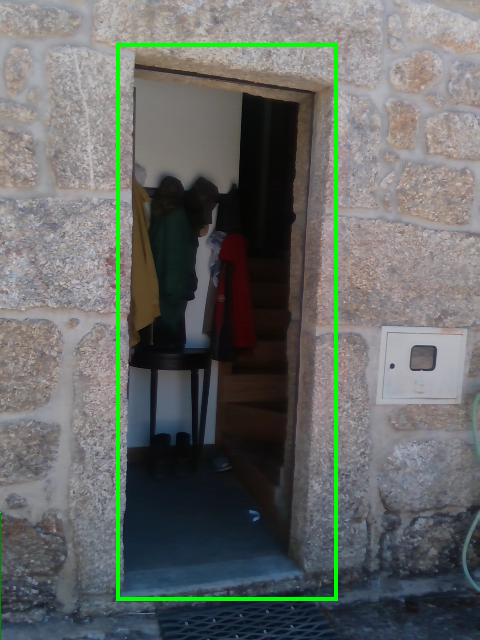
\includegraphics[width=\linewidth]{images/deep_doors_2_open.png}
		\caption{}
	\end{subfigure}
	\hfil
	\begin{subfigure}[b]{0.21\linewidth}
		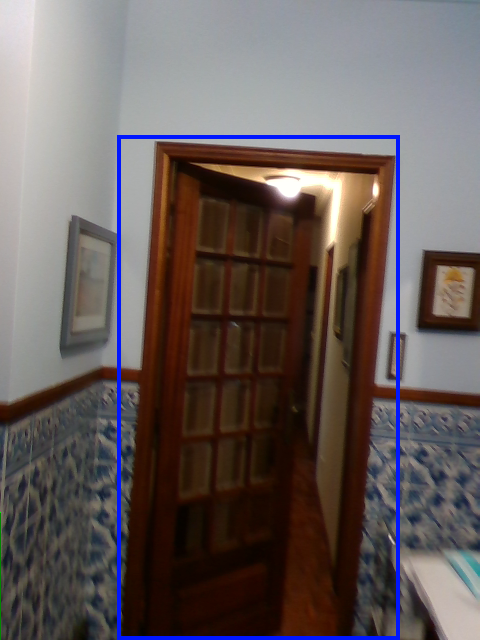
\includegraphics[width=\linewidth]{images/deep_doors_2_semiopen.png}
		\caption{}
	\end{subfigure}
	\hfil
	\begin{subfigure}[b]{0.21\linewidth}
		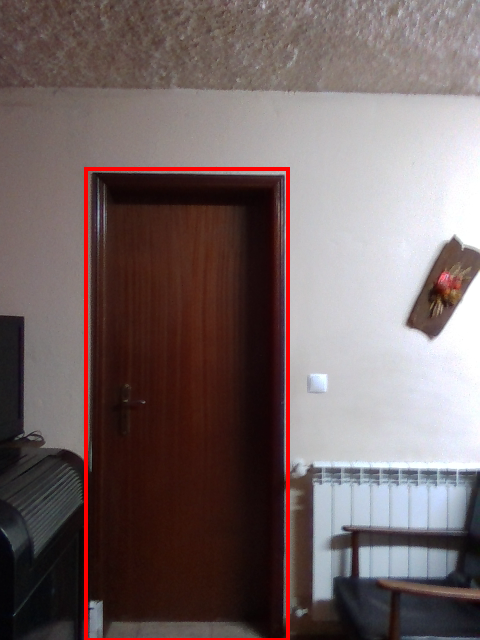
\includegraphics[width=\linewidth]{images/deep_doors_2_closed.png}
		\caption{}
	\end{subfigure}
	\hfil
	\caption{Labeled images from DeepDoors2 dataset. (a) An open door, (b) a semi-open door, and (c) a closed door. Green, blue, and red bounding boxes represent open, semi-open, and closed doors respectively.}
	\label{fig: open_semi_closed}
\end{figure}

The object detection part of DeepDoors2 dataset is annotated with an automatic procedure that finds bounding boxes around doors using the semantic data. The labeling algorithm implemented by the authors finds a single door for each image, but we argue that a single example can depict multiple doors instances with different statues (Fig. \ref{fig:relabeling_deepdoors2}). Due to this fact, we manually re-label the entire dataset with the visual tool described in Sec. \ref{sec:dataset_labeling}. Furthermore, we re-organize the dataset according to the standard defined by the \textit{generic-dataset} framework reported in Sec. \ref{sec:generic_dataset}. We release the re-labeled version of DeepDoors2 dataset\footnote{The DeepDoors2 re-labeled dataset can be downloaded \href{https://drive.google.com/file/d/1wSmFUHF9aSJkomwFdOmepMevBvkRpf3D/view?usp=sharing}{here}.} and the necessary Python code\footnote{The DeepDoors2 re-labeled source code: \url{https://github.com/micheleantonazzi/deep-doors-2-labelled}.} to manage it. The final DeepDoors2 dataset is composed of 2998 examples, while each of them includes an RGB image with dimension $480 \times 640 \times 3$, a matrix $480 \times 640$ which contains the depth data, and a list with the bounding boxes' coordinates and the relative labels (open, semi-open, or closed door). 

\begin{figure}[h!]
	\centering
	\begin{subfigure}[b]{\linewidth}
		\hfil
		\begin{subfigure}[b]{0.21\linewidth}
			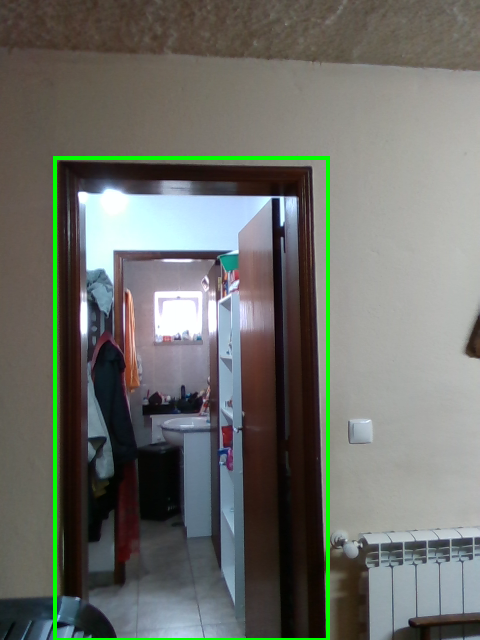
\includegraphics[width=\linewidth]{images/deep_doors_2_labeling1.png}
		\end{subfigure}
		\hfil
		\begin{subfigure}[b]{0.21\linewidth}
			
\includegraphics[width=\linewidth]{images/deep_doors_2_labeling1_semantic.png}
		\end{subfigure}
		\hfil
		\begin{subfigure}[b]{0.21\linewidth}
			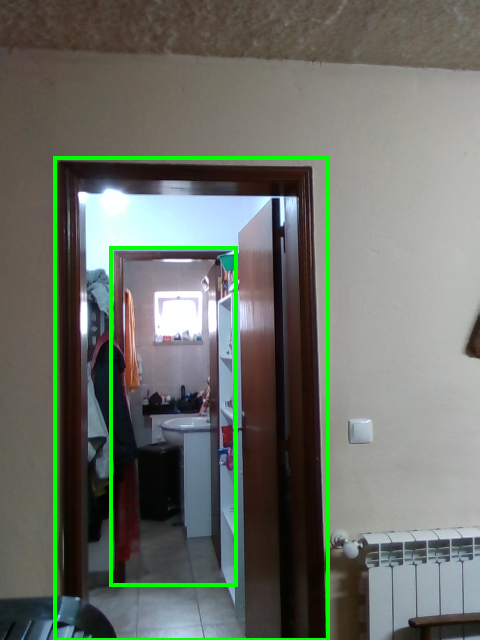
\includegraphics[width=\linewidth]{images/deep_doors_2_labeling1_correct.png}
		\end{subfigure}
		\hfil
		\caption{}
	\end{subfigure}
	\newline
	\begin{subfigure}[b]{\linewidth}
		\hfil
		\begin{subfigure}[b]{0.21\linewidth}
			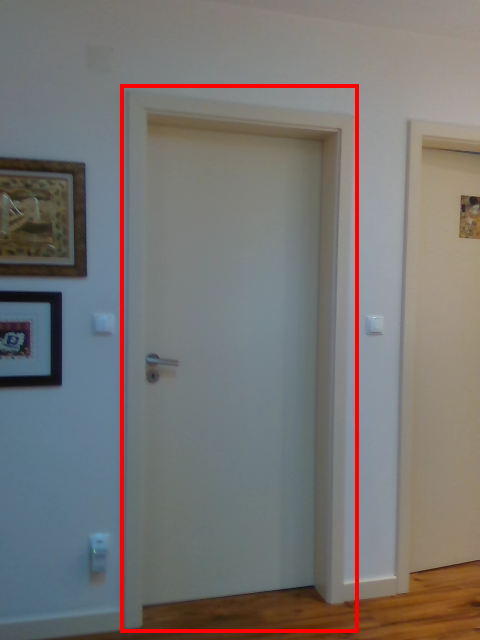
\includegraphics[width=\linewidth]{images/deep_doors_2_labeling2.png}
		\end{subfigure}
		\hfil
		\begin{subfigure}[b]{0.22\linewidth}
			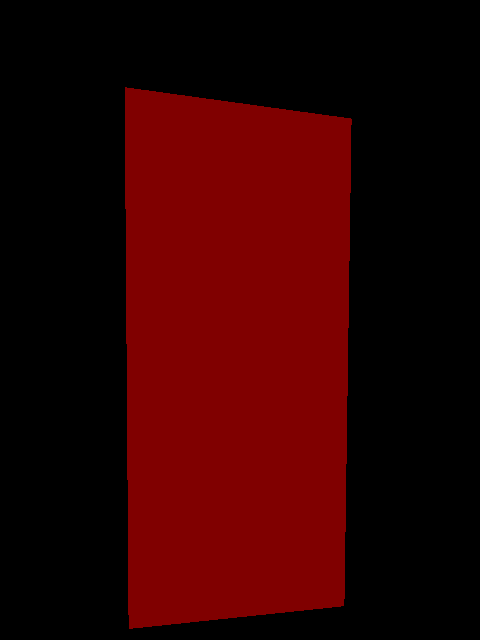
\includegraphics[width=\linewidth]{images/deep_doors_2_labeling2_semantic.png}
		\end{subfigure}
		\hfil
		\begin{subfigure}[b]{0.21\linewidth}
			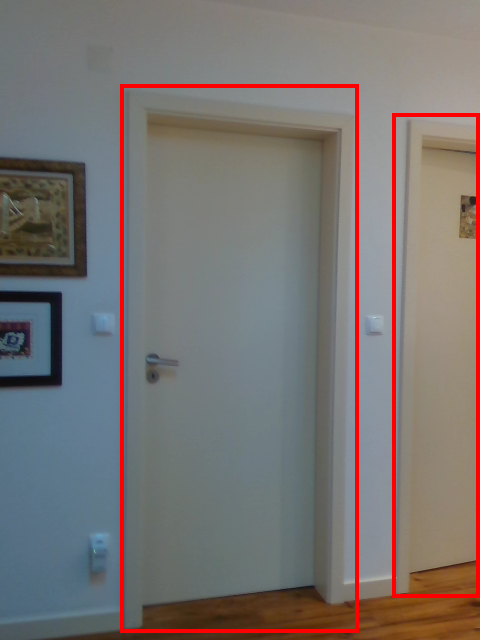
\includegraphics[width=\linewidth]{images/deep_doors_2_labeling2_correct.png}
		\end{subfigure}
	\hfil
		\caption{}
	\end{subfigure}
	\caption{Two examples of wrong labeled images from the original version of DeepDoors2 dataset. The left figures in each row represents the bounding boxes found with the depth data encoded in the middle images. The figures on the right depict the fixed labeled images of our version DeepDoors2.}
	\label{fig:relabeling_deepdoors2}
\end{figure}

\subsection{DETR's Performance on DeepDoors2}

Before proceeding with other experiments, we test DETR on the relabeled version of DeepDoors2 to verify if it converges with such a small dataset and if it has acceptable performance in a doors detection task. We randomly split the dataset into a training set with the $80\%$ of the examples and a test set with the remaining. We train DETR for 40 epochs with a batch size of 1. We report the DETR loss function (Eq. \ref{eq:detr_loss}) during training both for train and test sets in Fig. \ref{fig:deep_doors2_loss}.

\begin{figure}[h!]
	\centering
	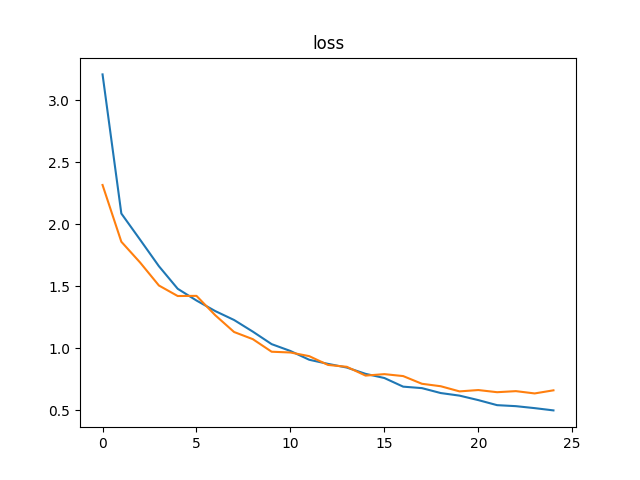
\includegraphics[width=\linewidth]{images/deep_doors_2_loss.png}
	\caption{The loss functions during the training of DETR.}
	\label{fig:deep_doors2_loss}
\end{figure}

We evaluate the trained version of DETR with the Pascal VOC metric \cite{pascal} as described in Sec. \ref{sec:model_evaluator}. We set the \textsf{iou\_threshold}$ = 0.9$ and the \textsf{confidence\_threshold} $= 0.5$. Table \ref{tab:deep_doors2_results} reports the AP score for each object category (open, semi-open, and closed doors) and the data to calculate it, such as the total number of the ground-truth bounding boxes, the true positive, and the false positive detections performed by the model. The plot of the interpolated precision/recall curves for each category is shown in Fig. \ref{fig:deep_doors2_ap_plot}.

\begin{table}[h!]
	\centering
	\begin{tabular}{cccccc}
		
		\toprule
		\textbf{Label} & \textbf{AP} & \textbf{N. Positives} & \textbf{TP} & \textbf{FP} & \textbf{FN}\tabularnewline
		\midrule
		Closed door (0) & 90 & 234 & 214 & 45 & 20 \tabularnewline
		Semi-open door (1) & 83 & 198 & 169 & 33 & 29 \tabularnewline
		Open door (2) & 85 & 243 & 214 & 66 & 29 \tabularnewline
		\bottomrule
	\end{tabular}
	\caption{The performance of DETR trained on the DeepDoors2 dataset.}
	\label{tab:deep_doors2_results}
\end{table}

\begin{figure}[h!]
	\centering
	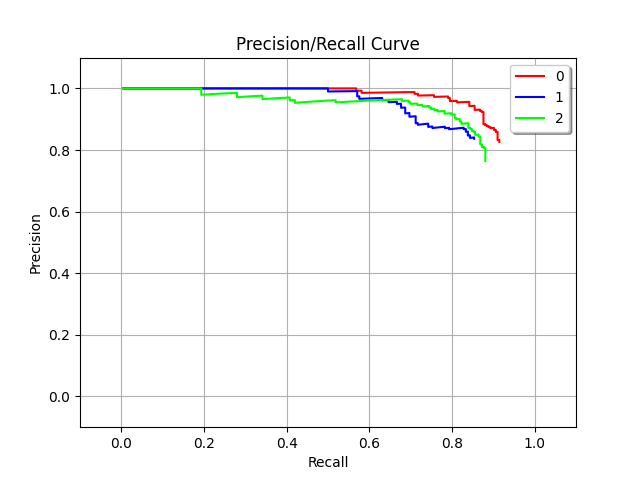
\includegraphics[width=0.93\linewidth]{images/deep_doors_2_precision_recall.png}
	\caption{The interpolated precision/recall curves about open, semi-open, and closes doors, colored in green, blue, and red respectively.}
	\label{fig:deep_doors2_ap_plot}
\end{figure} 

As shown by Fig. \ref{fig:deep_doors2_loss}, the model converges correctly and does not overfit or underfit. Both the training and test error (reported in blue and orange respectively) are low and closed to each other. As reported in Table \ref{tab:deep_doors2_results}, the proposed doors detector reaches a good detection accuracy for all the 3 door categories (open, semi-open, and closed). An AP greater than 80 is considered a good result in the Computer Vision community.

\subsection{The DETR's Detection Visualization}
As mentioned in Sec. \ref{sec:detrarchitecture}, each object query produces a detection composed of the bounding box coordinates and the relative label. To further analyze the DETR's performance, we plot in 2D the object queries classified by the Transformers using t-SNE \cite{tsne}. t-SNE (t-distributed Stochastic Neighbor Embedding) is a unsupervised and randomized technique to visualize high-dimensional data by giving each data point a location in a two or three dimensional map. This algorithm is a variation of Stochastic Neighbor Embedding (SNE) \cite{sne}. We plot the output embeddings of the Transformer with t-SNE in a two-dimensional space. We train DETR for 40 epochs with a batch size of 1 using 80\% of the examples of the re-labeled version of DeepDoors2. Then, we classify both the training set and the test set (composed the 20\% of the remaining examples) with the trained model, saving the object queries modified by the Transformer. Finally, we cluster only the predictions with the highest accuracy of every image using the \textit{scikit-image} implementation of t-SNE, by setting 2 different values for perplexity: 30 and 100. This hyper-parameter is a guess about the number of close neighbors each point has. Before clustering them through t-SNE, we reduce their dimensionality to 50 using the Principal Components Analysis (PCA) \cite{pca} algorithm, which projects a data point onto only the first few principal components preserving as much of the data's variation as possible. 

\begin{figure}[h!]
	\centering
	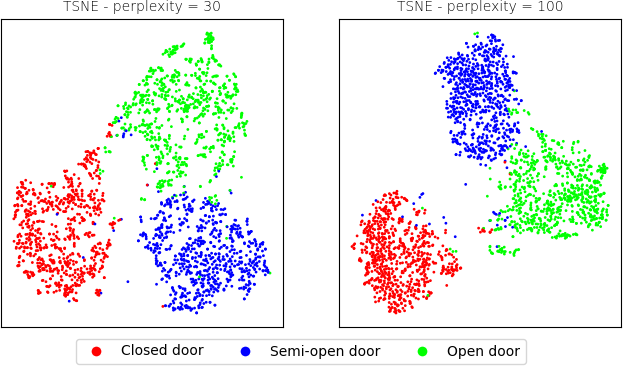
\includegraphics[width=\linewidth]{images/deep_doors_2_tsne_trainset.png}
	\caption{The plot of the Transformer's output embeddings using t-SNE over the training set.}
	\label{fig:tsne_deep_doors2_train}
\end{figure}

\begin{figure}[h!]
	\centering
	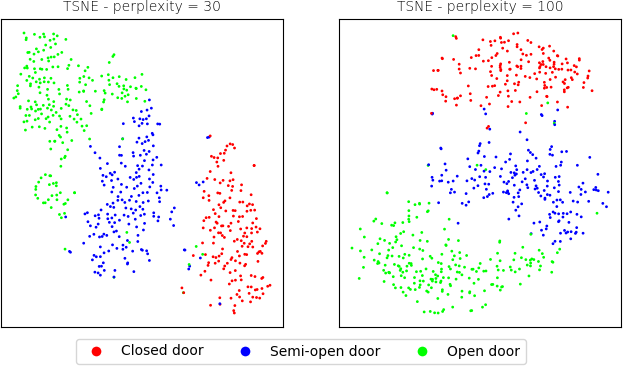
\includegraphics[width=\linewidth]{images/deep_doors_2_tsne_testset.png}
	\caption{The plot of the Transformer's output embeddings using t-SNE over the test set.}
	\label{fig:tsne_deep_doors2_test}
\end{figure}
 
The Figs. \ref{fig:tsne_deep_doors2_train} and \ref{fig:tsne_deep_doors2_test} show that DETR produces useful features encoding to separate the open, semi-open, and closed doors. Thanks to t-SNE, we argue that the objects queries classified by the Transformer are clearly separated into 3 distinct clusters examining both the training and the test sets (as expected looking at the good results reported in Tab. \ref{tab:deep_doors2_results}). Since the AP scores are not equal to 100, there are some spurious detections in the t-SNE's plots that likely lead to false positives.

\section{One-Shot Incremental Learning Evaluation}

As mentioned in Sec. \ref{sec:solution}, we not only offer a deep learning module for finding doors, but we also propose a technique for increasing the detector's performance exploiting a specific deployment scenario for a mobile robot as  explained in Sec. \ref{sec:deploymentscenario}. This technique, which we call \textbf{one-shot incremental learning}, consists on fine-tune a generic doors detector with a new dataset acquired directly from the new environment.
To successfully evaluate the \textbf{one-shot incremental learning} approach, the experimental phase of this thesis emulates the requirements for ideal deployment scenario for a mobile robot using the dataset of doors we collected. As reported in Sec. \ref{sec:dataset_acquisition}, the visual doors dataset has been acquired from set $E$ of 10 different environments from Matterport3D \cite{matterport} virtualized through the modified version of Gibson \cite{gibson} (described in Sec. \ref{sec:new_gibson_version}). The examples are both positive and negative and they are divided according to the environment of belonging. For each environment $e \in E$, the dataset $D_{e}$ (which contains the examples acquired from $e$) is split into 2 sub-sets $G_e$ and $S_e$, where $G_e$ contains all the examples that do not belong to the selected environment $e$, while $S_e$ is composed of the images collected from $e$. Then, $G_e$ is divided into 2 sub-sets $G^{P}_e$ and $G^{N}_e$: the first contains only the positive examples while the latter only the negative ones not acquired in the environment $e$. Likewise, $S_e$ is split in $S^{P}_e$ and $S^{N}_e$ that respectively contain the positive and the negative images of the environment $e$. Finally, 4 sub-sets are extracted from $S^{P}_e$, which are $S^{P}_{e, 1}$, $S^{P}_{e, 2}$, $S^{P}_{e, 3}$, and $S^{P}_{e, 4} $. They are composed of the 25\% of the examples of $S^{P}_e$. We use this dataset division to perform a series of two experiments for each environment:

\begin{itemize}
	\item \textbf{Experiment 1:} at first, we train for 40 epochs a general doors detector with $G^{P}_e$, that contains the positive examples that do not belong to the environment $e$. We use the configuration of DETR reported in Sec. \ref{sec:detr_configuration}. Then, we evaluate this model using the metric explained in Sec. \ref{sec:model_evaluator}, with a test set composed by $S^{P}_{e, 4}$ and $S^{N}_e$, that respectively contain the 25\% of the positive and all the negative image collected in $e$. We formally call this experiment \textsf{GD} (general doors detector). 
	
	\item \textbf{Experiment 2:} then, we perform a series of 3 fine-tune operations on the module trained in the previous experiment. We re-train (using the parameters reported in Sec. \ref{sec:detr_configuration}) for 20 epochs  the pre-trained module producing 3 fine-tuned versions of the generic doors detector using three different training sets $T$. At first, we set $ T= \big\{S^{P}_{e, 1}\big\}$, then $T=\big\{S^{P}_{e, 1} \cup S^{P}_{e, 2}\big\}$, and finally $T=\big\{S^{P}_{e, 1} \cup S^{P}_{e, 2} \cup S^{P}_{e, 3}\big\}$, so we fine-tune the general model by employing the  25\%, 50\%, and the 75\% of the positive samples collected in $e$. Like the previous experiment, each of the fine-tuned doors detector is evaluated through the metric described in Sec. \ref{sec:model_evaluator} using the remaining 25\% of the positive examples and all the negative images, contained in $S^{P}_{e, 4}$ and $S^{N}_e$ respectively. We refer to these 3 fine-tuned detectors as \textsf{FD\textsubscript{25}}, \textsf{FD\textsubscript{50}}, and \textsf{FD\textsubscript{75}}. 

\end{itemize}

In simple terms, we built 4 different doors detector for each environment in the collected dataset: the general doors detector (\textsf{GD}) is trained without images acquired in the selected environment, and other 3 detectors trained by fine-tuning the general model with the 25\% (\textsf{FD\textsubscript{25}}), 50\% (\textsf{FD\textsubscript{50}}), and 75\% (\textsf{FD\textsubscript{75}}) of the examples of the selected environment. All these models are tested with the remaining 25\% of the samples of the current environment ($S^{P}_{e,4}$) and all the negative images of the current environment ($S^{N}_{e}$).

\subsection{Detail Results in One Example Environment}

Before proceeding with a complete analysis of the proposed method using all the environments in $E$, we report a detailed study of a single environment from Matterport3D \cite{matterport}, \textsf{house13}. First of all, we test the performance of the trained detectors (the general detector \textsf{GD} and the 3 fine-tuned models \textsf{FD\textsubscript{25}}, \textsf{FD\textsubscript{50}}, and \textsf{FD\textsubscript{75}}) using the metric explained in Sec. \ref{sec:model_evaluator}. Table \ref{tab:house13_results} shows the results obtained with \textsf{house13}, reporting the AP scores and the increment in percentage of AP between each experiment and the previous one. The AP values are computer on a test set $T = S^{P}_{e, 4} \cup S^{N}_{e}$, which contains the 25\% of positive and all the negative examples collected in $e$. The values contained in this table are plotted in Fig. \ref{fig:house13_AP_results}, which reports the AP scores grouped by label in order to visualize the AP change from one experiment to the next. We set the metric's hyper-parameters at 0.5 and 0.75 for the \textsf{confidence\_threshold} and \textsf{iou\_threshold} respectively.

\begin{table}[h!]
	\centering
	\begin{tabular}{ccccc}
		
		\toprule
		\textbf{Env.} & \textbf{Exp.} & \textbf{Label} & \textbf{AP} & \textbf{Increment}  \\
		\midrule
		\multicolumn{1}{c|}{\multirow{12}{*}{House 13}} & \multicolumn{1}{c|}{\multirow{3}{*}{\textsf{GD}}} & No door (-1) & 68 & -  \tabularnewline 
		\multicolumn{1}{c|}{}& \multicolumn{1}{c|}{} & Closed door (0) & 66 & -  \\
		\multicolumn{1}{c|}{}& \multicolumn{1}{c|}{}& Open door (1) & 64 & -  \\  \cline{2-5}
		\multicolumn{1}{c|}{}& \multicolumn{1}{c|}{\multirow{3}{*}{\textsf{FD\textsubscript{25}}}} & No door (-1) & 74 & $+8\%$  \tabularnewline [1pt]
		\multicolumn{1}{c|}{}& \multicolumn{1}{c|}{} & Closed door (0) & 74 & $+13\%$  \\ 
		\multicolumn{1}{c|}{}& \multicolumn{1}{c|}{} & Open door (1) & 67 & $+4\%$   \\ \cline{2-5}
		\multicolumn{1}{c|}{} & \multicolumn{1}{c|}{\multirow{3}{*}{\textsf{FD\textsubscript{50}}}} & No door (-1) & 76 & $+2\%$  \tabularnewline 
		\multicolumn{1}{c|}{}& \multicolumn{1}{c|}{} & Closed door (0) & 84 & $+14\%$  \\
		\multicolumn{1}{c|}{}& \multicolumn{1}{c|}{}& Open door (1) & 76 & $+13\%$  \\  \cline{2-5}
		\multicolumn{1}{c|}{}& \multicolumn{1}{c|}{\multirow{3}{*}{\textsf{FD\textsubscript{75}}}} & No door (-1) & 79 & $+4\%$  \tabularnewline [1pt]
		\multicolumn{1}{c|}{}& \multicolumn{1}{c|}{} & Closed door (0) & 83 & $-2\%$  \\ 
		\multicolumn{1}{c|}{}& \multicolumn{1}{c|}{} & Open door (1) & 73 & $-4\%$   \\ 
		\bottomrule
	\end{tabular}
	\caption{The evaluation of the \textbf{one-shot incremental learning} on \textsf{house13}. This table reports the AP scores obtained by the 4 doors detectors on 3 labels: negative bounding box (predicted in the negative images), closed doors, and open doors. In addition, the last column shows the increments obtained by the 3 fine-tune operations.}
	\label{tab:house13_results}
\end{table}

\begin{figure}[h!]
	\centering
	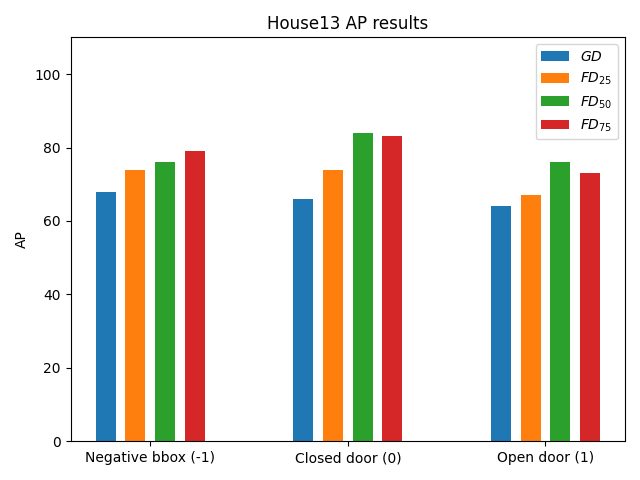
\includegraphics[width=0.86\linewidth]{images/house13_AP_results.png}
	\caption{The AP score obtained in the experiments of \textsf{house13} grouped by label (negative bounding box, closed door, and open door).}
	\label{fig:house13_AP_results}
\end{figure}

Then, we report the plots of the loss functions (Eq. \ref{eq:detr_loss}) during the training of the 4 doors detectors (Fig. \ref{fig:house13_losses}). The training loss is the average of the loss value computed with the training data during each epoch, while the test loss is calculated at the end of each epoch using all the positive examples ($S^{P}_e$) in the general detector and the 25\% of positive images (which corresponds to the $S^{P}_{e,4}$ sub-set) for the 3 fine-tuned models.

\begin{figure}[h!]
	\centering
	\begin{subfigure}[b]{0.49\linewidth}
		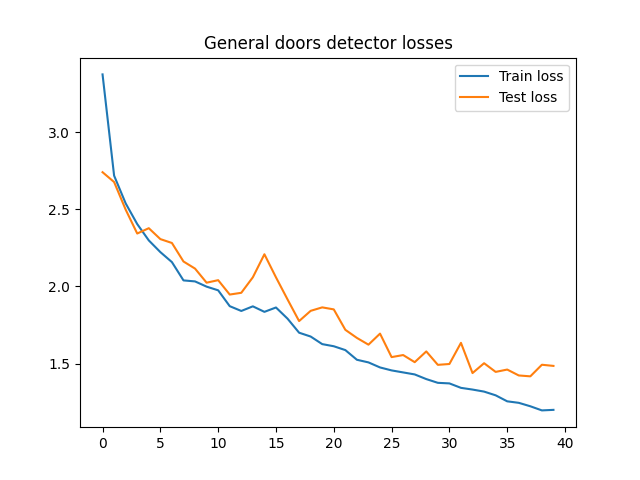
\includegraphics[width=\linewidth]{images/house13_general_detector_loss.png}

	\end{subfigure}
	\hfil
	\begin{subfigure}[b]{0.49\linewidth}
		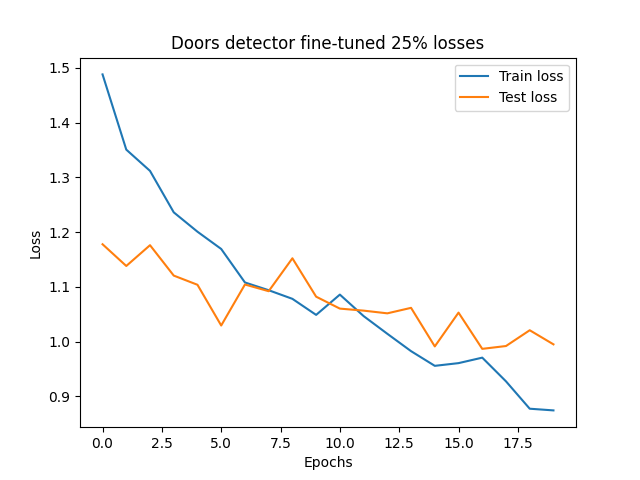
\includegraphics[width=\linewidth]{images/house13_finetune25_loss.png}

	\end{subfigure}
	\newline
	\newline
	\begin{subfigure}[b]{0.49\linewidth}
		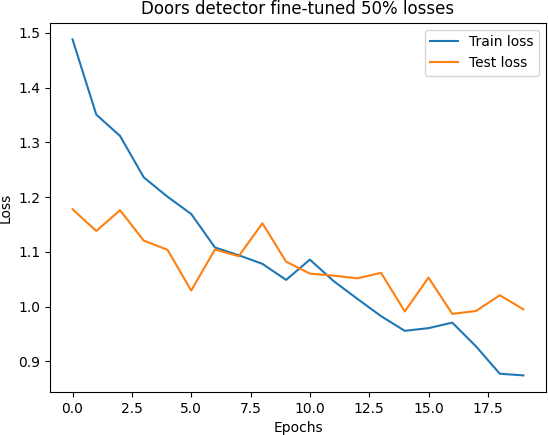
\includegraphics[width=\linewidth]{images/house13_finetune50_loss.png}

	\end{subfigure}
	\hfil
	\begin{subfigure}[b]{0.49\linewidth}
		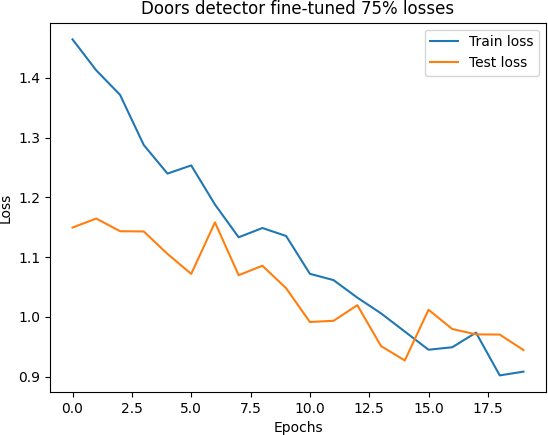
\includegraphics[width=\linewidth]{images/house13_finetune75_loss.png}

	\end{subfigure}
	\caption{The losses values of DETR during the training on \textsf{house13}. }
	\label{fig:house13_losses}
\end{figure}

The first consideration is that the configuration of DETR (reported in Sec. \ref{sec:detr_configuration}) allows  a correct training of all the model versions (\textsf{GD}, \textsf{FD\textsubscript{25}}, \textsf{FD\textsubscript{50}}, and \textsf{FD\textsubscript{75}}). As shown in Fig. \ref{fig:house13_losses}, both the training and test losses decrease to 0 and are close to each other. 

By examining the table reporting the AP score (Tab \ref{tab:deep_doors2_results}), we argue that our door detector achieves good performance even with a general train (without using any examples of {house13}). In fact, the \textsf{GD} detector reaches 68, 66, and 64 of AP for negative bounding boxes, closed doors, and open doors respectively. The fine-tune operations tend to increase the doors detector's performance. In particular, the first fine-tuned detector (\textsf{FD\textsubscript{25}}) increases the AP by a factor of 8\%, 13\%, and 4\% for the negative bounding boxes, closed doors, and open doors respectively. Also the \textsf{FD\textsubscript{50}} module increase a lot the doors detector's performance. More precisely, by a factor of 2\%, 14\%, and 13\% for negative bounding boxes, closed doors, and open doors respectively. Surprisingly, the detector fine-tuned with the 75\% of the positive examples of \textsf{house13} degrades the AP scores for both open and closed doors. As shown in Fig. \ref{fig:house13_AP_results}, the AP score of the negative bounding boxes increases in all experiments, but, for the closed and open doors, the AP value significantly grows up only in the \textsf{FD\textsubscript{25}} and \textsf{FD\textsubscript{50}}, while it goes down in the last fine-tuned detector (\textsf{FD\textsubscript{75}}).

\subsection{Results Over All Environments}

After the analysis of the \textbf{one-shot incremental learning} behavior considering a single environment (\textsf{house13}), we evaluate such a technique on the entire visual dataset collected in this thesis. As a reminder, the dataset has been acquired from a set $E$ composed of 10 environments of Matterport3D \cite{matterport}: \textsf{house1}, \textsf{house2}, \textsf{house7}, \textsf{house9}, \textsf{house10}, \textsf{house13}, \textsf{house15}, \textsf{house20}, \textsf{house21},  \textsf{house22}.
For each environment $e \in E$, we train 4 door detectors. The first (\textsf{GD}) is trained with all the examples of the dataset except those collected in the selected environment ($G^{P}_e$). Then, we fine-tune 3 times the general model with the 25\%, 50\%, and 75\% of the positive examples from $e$,  producing 3 fine-tuned detectors: \textsf{FD\textsubscript{25}}, \textsf{FD\textsubscript{50}}, and \textsf{FD\textsubscript{75}}. We perform their  evaluation using the metric describe in Sec. \ref{model_evaluator}, setting \textsf{iou\_threshold} $= 0.75$ and the \textsf{confidence\_threshold} $= 0.50$. The AP values are calculated using a fixed test set $T = S^{P}_{e, 4} \cup S^{N}_{e}$, composed by the 25\% of positive and all the negative examples collected in $e$.  We report the mean of the AP scores reached by the 4 detectors divided by label (negative bounding boxes, closed door, and open door), the increments' average obtained with the fine-tune operations, and the standard deviation ($\sigma$) of both of them in Table \ref{tab:all_houses_results}. We also report the AP scores of all environments in two plots. In particular, Fig. \ref{fig:all_houses_closed} depicts the AP scores reached by the general and the 3 fine-tuned detectors on closed doors, while in Fig. \ref{fig:all_houses_open} are reported the detectors' performance on open doors. The environments are increasing ordered based on the AP score obtained with the \textsf{FD\textsubscript{25}} doors detector.

\begin{table}[h!]
	\centering
	\begin{tabular}{ccccccc}
		
		\toprule
		\textbf{Env.} & \textbf{Exp.} & \textbf{Label} & \textbf{AP} & \textbf{$\sigma$} & \textbf{Increment} &  \textbf{$\sigma$} \\
		\midrule
		\multicolumn{1}{c|}{\multirow{12}{*}{All houses}} & \multicolumn{1}{c|}{\multirow{3}{*}{\textsf{GD}}} & No door (-1) & 74 & 5 & - & - \tabularnewline 
		\multicolumn{1}{c|}{}& \multicolumn{1}{c|}{} & Closed door (0) & 39 & 14 & - & -  \\
		\multicolumn{1}{c|}{}& \multicolumn{1}{c|}{}& Open door (1) & 60 & 8 & - & -  \\  \cline{2-7}
		\multicolumn{1}{c|}{}& \multicolumn{1}{c|}{\multirow{3}{*}{\textsf{FD\textsubscript{25}}}} & No door (-1) & 79 & 4 & $+7\%$ & $9\%$ \tabularnewline [1pt]
		\multicolumn{1}{c|}{}& \multicolumn{1}{c|}{} & Closed door (0) & 61 & 10 &  $+75.5\%$ & $66\%$  \\ 
		\multicolumn{1}{c|}{}& \multicolumn{1}{c|}{} & Open door (1) & 70 & 7 & $+16\%$ & $14\%$  \\ \cline{2-7}
		\multicolumn{1}{c|}{} & \multicolumn{1}{c|}{\multirow{3}{*}{\textsf{FD\textsubscript{50}}}} & No door (-1) & 78 & 5 & $-1\%$ & $5\%$  \tabularnewline 
		\multicolumn{1}{c|}{}& \multicolumn{1}{c|}{} & Closed door (0) & 69 & 12 & $+13\%$ & $9\%$ \\
		\multicolumn{1}{c|}{}& \multicolumn{1}{c|}{}& Open door (1) & 73 & 6 & $+5\%$ & $5\%$ \\  \cline{2-7}
		\multicolumn{1}{c|}{}& \multicolumn{1}{c|}{\multirow{3}{*}{\textsf{FD\textsubscript{75}}}} & No door (-1) & 79 & 5 & $+1\%$ & $4\%$  \tabularnewline [1pt]
		\multicolumn{1}{c|}{}& \multicolumn{1}{c|}{} & Closed door (0) & 72 & 11 & $+6\%$ & $10\%$  \\ 
		\multicolumn{1}{c|}{}& \multicolumn{1}{c|}{} & Open door (1) & 76 & 6 & $+5\%$ & $5\%$  \\ 
		\bottomrule
	\end{tabular}
	\caption{The evaluation of the \textbf{one-shot incremental learning} over the entire dataset. This table reports the mean of the AP scores of the 4 doors detectors on the 3 labels: negative bounding box (predicted in the negative images), closed doors, and open doors, showing also the  the increments' average obtained by the 3 fine-tune operations. In addition, we report the standard deviations for the AP scores and the relative increments.}
	\label{tab:all_houses_results}
\end{table}

\begin{figure}[h!]
	\centering
		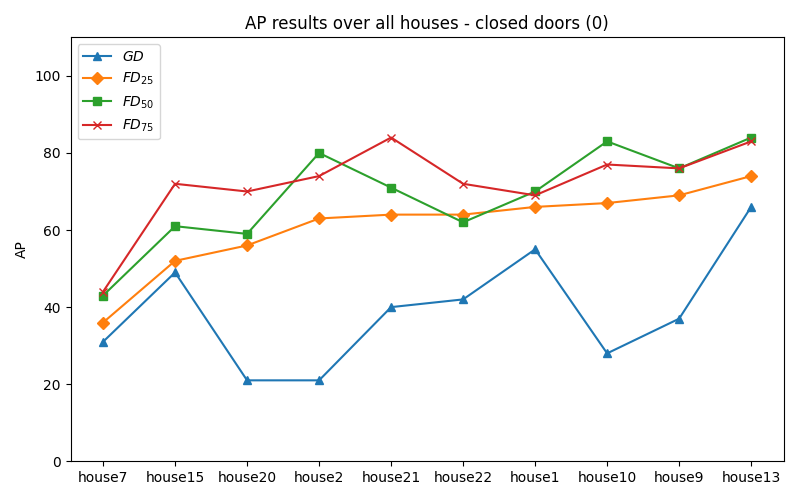
\includegraphics[width=\linewidth]{images/all_houses_results_closed.png}
	\caption{The AP scores obtained by the 4 doors detectors' versions (\textsf{GD}, \textsf{FD\textsubscript{25}}, \textsf{FD\textsubscript{50}}, and \textsf{FD\textsubscript{75}}) over the entire dataset on closed doors, grouped by environment. }
	\label{fig:all_houses_closed}
\end{figure}

\begin{figure}[h!]
	\centering
	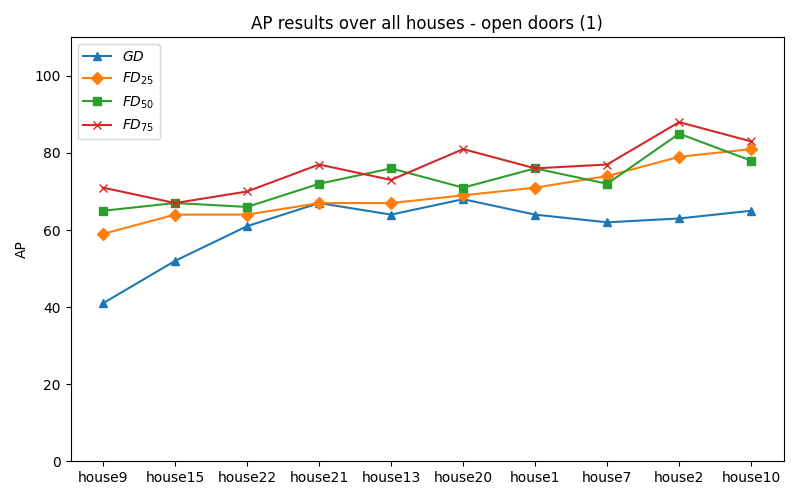
\includegraphics[width=\linewidth]{images/all_houses_results_open.png}
	\caption{The AP scores obtained by the 4 doors detectors' versions (\textsf{GD}, \textsf{FD\textsubscript{25}}, \textsf{FD\textsubscript{50}}, and \textsf{FD\textsubscript{75}}) over the entire dataset on open doors, grouped by environment.}
	\label{fig:all_houses_open}
\end{figure}

The results reported in Table \ref{tab:all_houses_results} shows that our doors detector obtains, in average, good AP scores for all the considered labels even if it is trained in a general way (without considering the examples of the selected environment). The \textsf{GD} detector recognizes negative bounding boxes, closed doors, and open doors with average AP scores of 74, 39, and 60 respectively. By observing the increment values, we argue that the fine-tuned versions of the general doors detectors increase in average the detection accuracy on all classes with respect to the previous steps. The unique exception is for the negative bounding boxes in \textsf{FD\textsubscript{50}} detectors, where the average AP score decreases by 1\%.  The table shows that the first fine-tune operation (in which the general detectors are trained with the 25\% of the examples collected from a certain environment) gives the highest increment in performance. The closed doors, which is the category worst recognized by the general detectors, reaches a mean AP of 61, with a growth of 75\%. The AP averages of the open doors and the negative bounding boxes reach the values of 70 and 79 respectively, with an increment of 16\% and 7\%. The subsequent fine-tune operations (\textsf{FD\textsubscript{50}} and \textsf{FD\textsubscript{75}}) increase the average detection accuracy on all labels (except for negative bounding boxes in \textsf{FD\textsubscript{50}}) but in much smaller increments with respect to the fine-tune with only the 25\% of examples. 

Figs. \ref{fig:all_houses_closed} and \ref{fig:all_houses_open} allow us to better evaluate the impact of the \textbf{one-shot incremental learning} approach applied to all the environments in the collected dataset. They clearly show that the performance of the general detectors over the closed doors is extremely variable (as shown by the standard deviations in Table \ref{tab:all_houses_results}) and, sometimes, the closed doors are detected with an AP less than 30 (for example in \textsf{house2}, \textsf{house10}, and \textsf{house20}). At best of our knowledge, this fact can be caused by two factors. The first is the dataset's imbalance: the closed doors' examples are significantly less than open doors' images. For example, \textsf{house2} has 155 images of open doors but only 30 of closed doors. The second reason is the features that characterize the closed doors. Such a door category is stronger to be detected because it often blends with the surrounding wall. Otherwise, the doors detector works well with open doors because they expose more clear features. These figures confirm that fine-tuning a general doors detector with the 25\% of examples collected in a specific environment assure the best performance increasing with respect to the subsequent fine-tunes for both open and closed doors. Despite the \textsf{FD\textsubscript{75}} detectors reach in average the best performance, for many environments this is not true. For example, considering the open doors, in \textsf{house15} and \textsf{house1} fine-tuning with the 75\% of examples does not increase the module's performance, while in \textsf{house13} \textsf{FD\textsubscript{75}} degrades the detection accuracy with respect to \textsf{FD\textsubscript{50}}. Likewise, fine-tuning with the 50\% of the positive examples generally increase the performance with respect to the previous steps, but this fact is not confirmed by \textsf{house7} and \textsf{house10} considering the open doors.

The results reported in this section show that the collected dataset is more challenging than DeepDoors2 \cite{deepdoors2} and it is more suitable for evaluating a detector of doors used by a mobile robot. This is because it allows reproducing the deployment scenario described in Sec. \ref{sec:deploymentscenario}. The examples are divided according to the environment from which they belong, so it allows to evaluate the detection accuracy of an end-to-end module for finding doors considering multiple environments with different doors types. Furthermore, our dataset contains also negative images to model the typical uncertainty in which a robot operates. 

The collected results show also that our doors detector, built using DETR \cite{detr}, is able to detect doors in a new environment with variable performance (especially the challenging category of closed doors). We demonstrate that the \textbf{one-shot incremental learning} is a valid approach for increasing the performance of a general doors detector to specialize in a specific environment. We also argue that a little fine-tune operation, considering the 25\% of examples of a new environment, is enough to obtain a significant performance improvement also for the more challenging environments. This is shown by Fig. \ref{fig:all_houses_closed}, where the AP scores over the closed doors significantly grow up from \textsf{GD} to \textsf{FD\textsubscript{25}} on \textsf{house2} and \textsf{house10}.



